%%%%%%%%%%%%%%%%%%%%%%%%%%%%%%%%%%%%%%%%%
% scelta_delle_classi.tex v1.0
%
% Relazione per il progetto PuzzleSolver (Parte 2)
% Autore: Giacomo Cusinato
% Materia: Programmazione Concorrente e Distribuita
%
%%%%%%%%%%%%%%%%%%%%%%%%%%%%%%%%%%%%%%%%%

\section{Differenze con la versione precedente}
Il progetto non ha subito molte variazioni rispetto alla versione precedente in quanto le operazioni effettuate dall'algorimo scelto sono
risultate facilmente portabili ad un'architettura concorrente. Di seguito sono riportate le modifiche effettuate alla classe principale,
contentente l'algorimo di risoluzione, ed una descrizione della nuova classe \texttt{PuzzleThread}.


\subsection{La classe PuzzleThread}
La classe \texttt{PuzzleThread} definisce un un oggetto la cui istanza può essere lanciata dal programma in un thread a supporto della risoluzione dell'algorimo.
La classe implementa l'interfaccia \texttt{Runnable} che rappresenta l'attività logica eseguibile dal thread e con cui è possibile creare oggetti di tipo \texttt{Thread}.
È stato scelto di implementare tale interfaccia invece che estendere la classe \texttt{Thread} dato che l'unico scopo della classe in questione è quello di effettuare
l'override del metodo \texttt{run()} per definire la logica eseguibile, metodo implementato appunto da \texttt{Runnable}, scelta che aumenta inoltre l'estensibilità
del classe considerato il vincolo di ereditarietà multipla in Java.
La classe è composta del seguente costruttore e metodo:
\begin{itemize}
    \item \texttt{public PuzzleThread(int, PuzzleSolver)}: il costruttore della classe accetta come parametri formali un intero, che indica la riga del puzzle dove il
    thread andrà ad operare, e l'istanza dell'oggetto di tipo \texttt{PuzzleSolver}, che espone il metodo principale per riordinare la riga. Entrambi i valori vengono
    memorizzati in due campi dati, entrambi utilizzati dal metodo \texttt{run()}.
    \item \texttt{public void run()}: è il metodo dichiarato dell'interfaccia \texttt{Runnable} che sarà lanciato una volta in esecuzione il thread. Si occupa di chiamare
    il metodo \texttt{reoderRow()}, illustrato in seguito, utilizzato dall'oggetto di tipo \texttt{PuzzleSolver} per ordinare una determinata riga del puzzle.
\end{itemize}



\subsection{La classe \texttt{PuzzleSolver}}
La classe \texttt{PuzzleSolver} è la classe di riferimento del programma, ovvero quella che contiene l'algorimo di risoluzione ed elabora
i dati in accesso ed uscita.


\subsubsection{L'algoritmo di risoluzione}
L'algorirmo di risoluzione presenta essenzialmente lo stesso funzionamento di quello illustrato nella precedente relazione, sebbene sia sia stato reso parallelo
attraverso la creazione di un thread per ogni riga del puzzle.
Il thread principale, come spiegato in precedenza, si occupa di riempire la prima colonna del puzzle così da avere un punto di partenza per i threads, ognuno dei
quali si occupera di terminare l'ordinamento di ciascuna riga.
Ogni thread opera in una singola ed unica riga del puzzle, proprio per questo non è stato necessario gestire l'utilizzo di risorse condivise tramite i costrutti
di cui dispone Java.


\subsubsection{Il metodo \texttt{void reoderRow(int row)}}
Il metodo \texttt{reoderRow(int row)} ha la funzione di riordinare un riga del puzzle, rappresentato da un array bidimensionale.
\`{E} il metodo utilizzato da ogni thread per accedere al puzzle ed ordinare la riga desidarata  grazie all'instanza di \texttt{PuzzleSolver}
passata come parametro formale al costruttore dell'oggetto di tipo \texttt{PuzzleThread}.


\subsubsection{L'utilizzo del Thread Pool}
La creazione di un thread per ogni riga è una scelta che può causare un utilizzo di memoria particolarmente elevato e basse performance, in particolar modo durante la manipolazione
di puzzle a dimensioni elevate.
Il pool di thread è un modulo che permette la gestione di più di thread creando una coda di task in esecuzione o in attesa in modo da limitare il più possibile
l'overhead causato dalla creazione ed esecuzione dei thread.
In supporto all'algorimo di risoluzione, quindi, è stato scelto di utizzare un \texttt{FixedThreadPool}, un tipo di thread pool che fissa un massimo numero di thread
operanti in contemporanea e gestisce in automatico tutti i task assegnati in attesa.

\begin{figure}[htbp]
    \centering
    \centerline{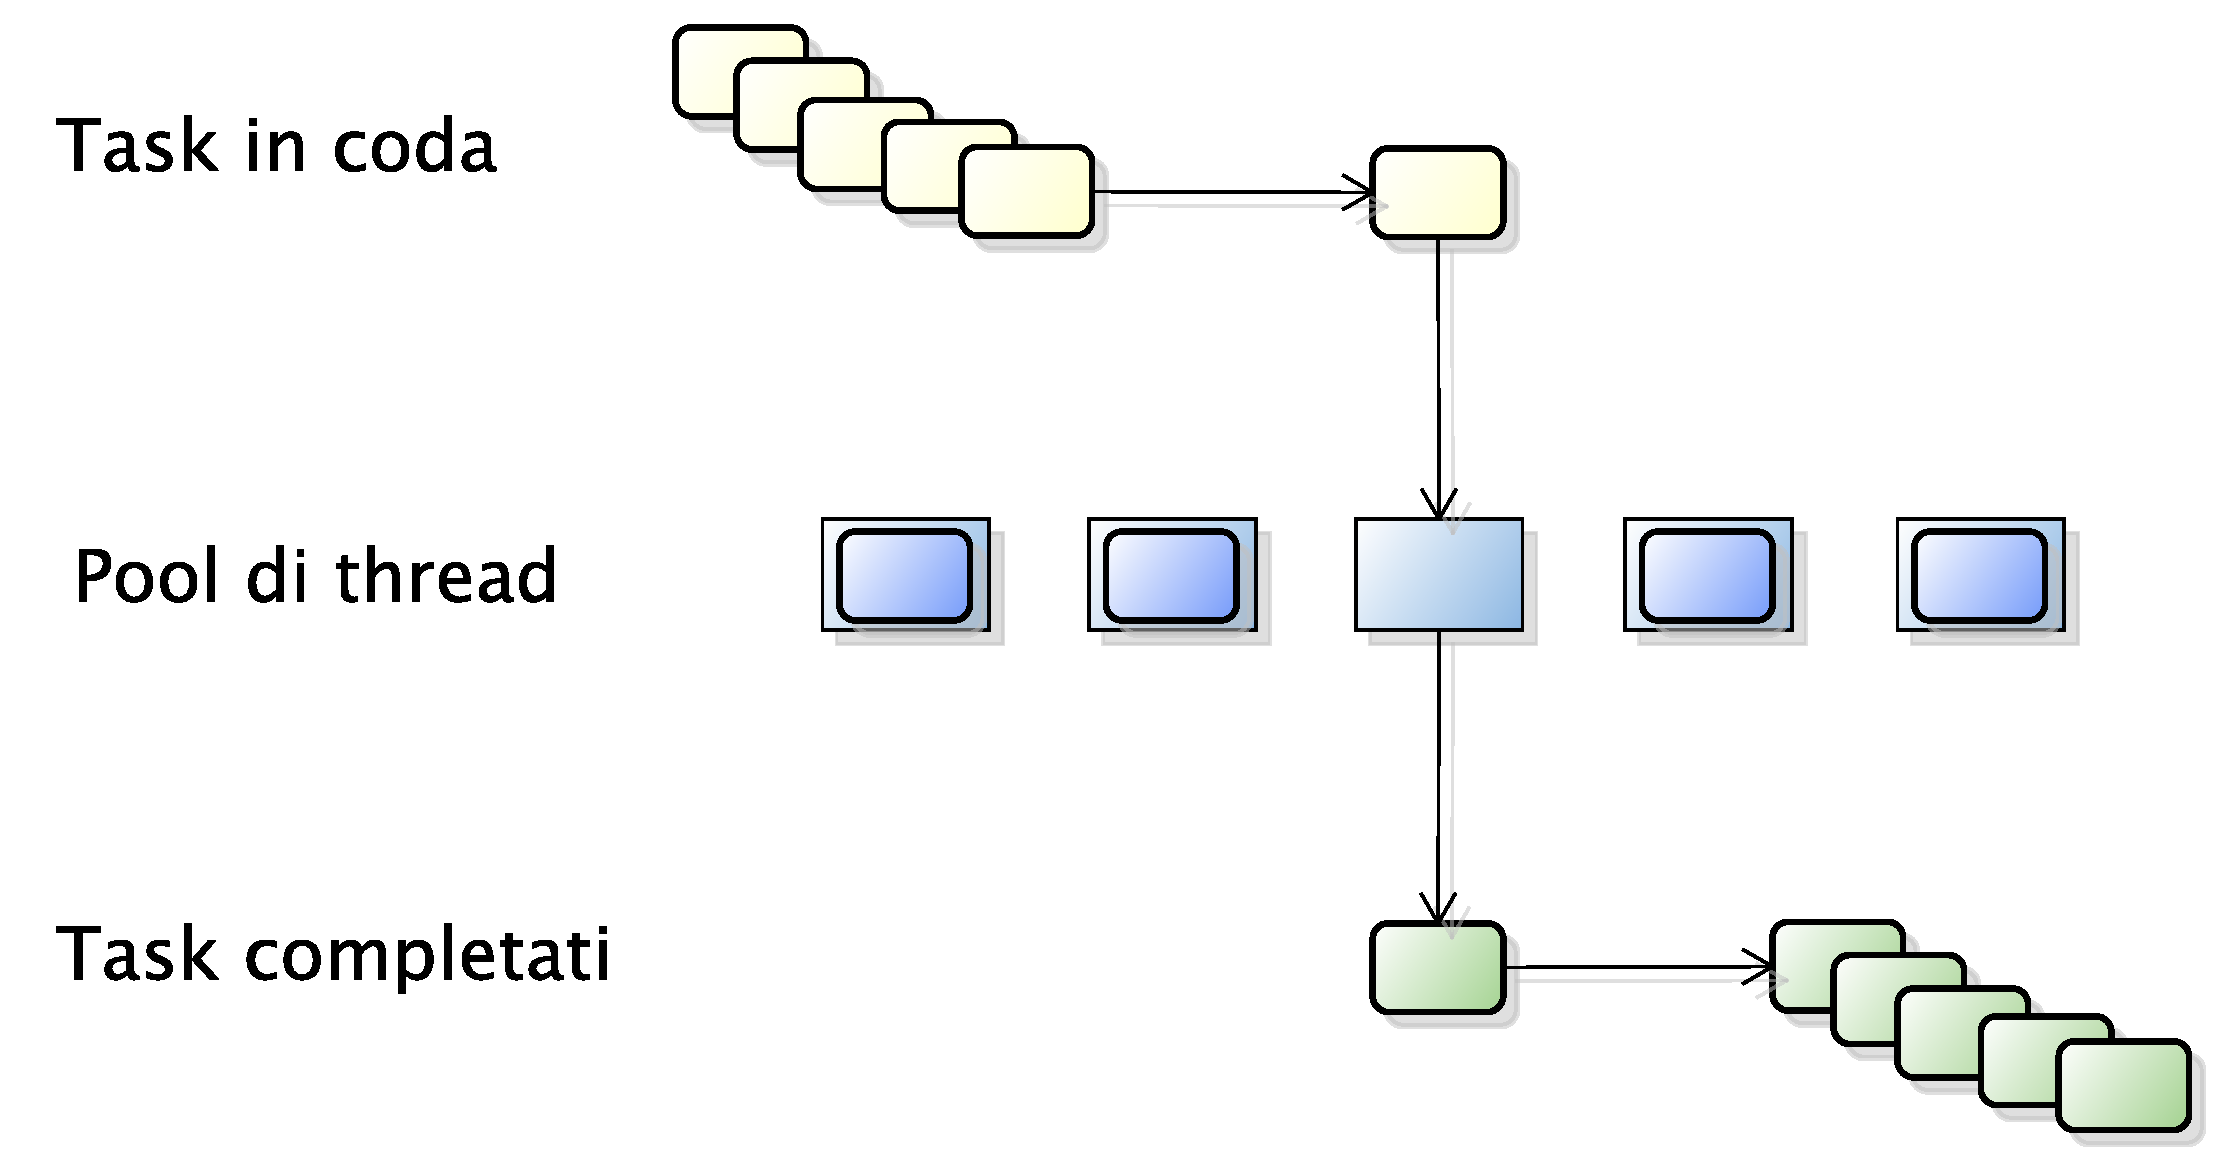
\includegraphics[scale=0.4]{./images/threadpool.pdf}}
    \caption{Thread Pool con 5 thread fissi}
\end{figure}

Il metodo \texttt{reorder()} della classe \texttt{PuzzleSolver} utilizza un oggetto di tipo \texttt{ExecutorService} per gestire un pool di 5 thread fissi, costruito tramite il metodo statico \texttt{newFixedPoolThread(5)}.
In questo modo è possibile creare un oggetto di tipo \texttt{PuzzleThread} per ogni riga e passare l'istanza creata al pool di thread tramite il metodo \texttt{execute()}.
Il thread pool gestisce ora in automatico la coda dei task e l'esecuzione di un thread non appena un altro in esecuzione termina il metodo \texttt{run()}.
Una volta assegnati tutti i task, viene invocato il metodo \texttt{shutdown()} per terminare il thread pool una volta completati tutti i task, situazione che si verificherà al termine del successivo ciclo while,
che assicura il completamento di tutti i task di riordinamento prima di proseguire con le  istruzioni del thread principale. In questo modo si ha la certezza di ricevere il puzzle completato prima di utilizzare
l'array ordinato per restituire il risultato del programma.
